\chapter{Analysis}

\section{Environment}

\subsection{Abalone rules}
The goal of the game is to push six of the opponent's marbles off the playing field. The game's starting position is depicted in figure \ref{basics} (a). One, two, or three adjacent marbles (of the player's own color) may be moved in any of the six possible directions during a player's turn. We differentiate between broadside or "side-step" moves and "in-line" moves, depending on how the chain of marbles moves relative to its direction, which is shown in figure \ref{basics} (b) and (c).

\begin{figure}[!h]
    \centering
    \subfloat[Starting position]{
        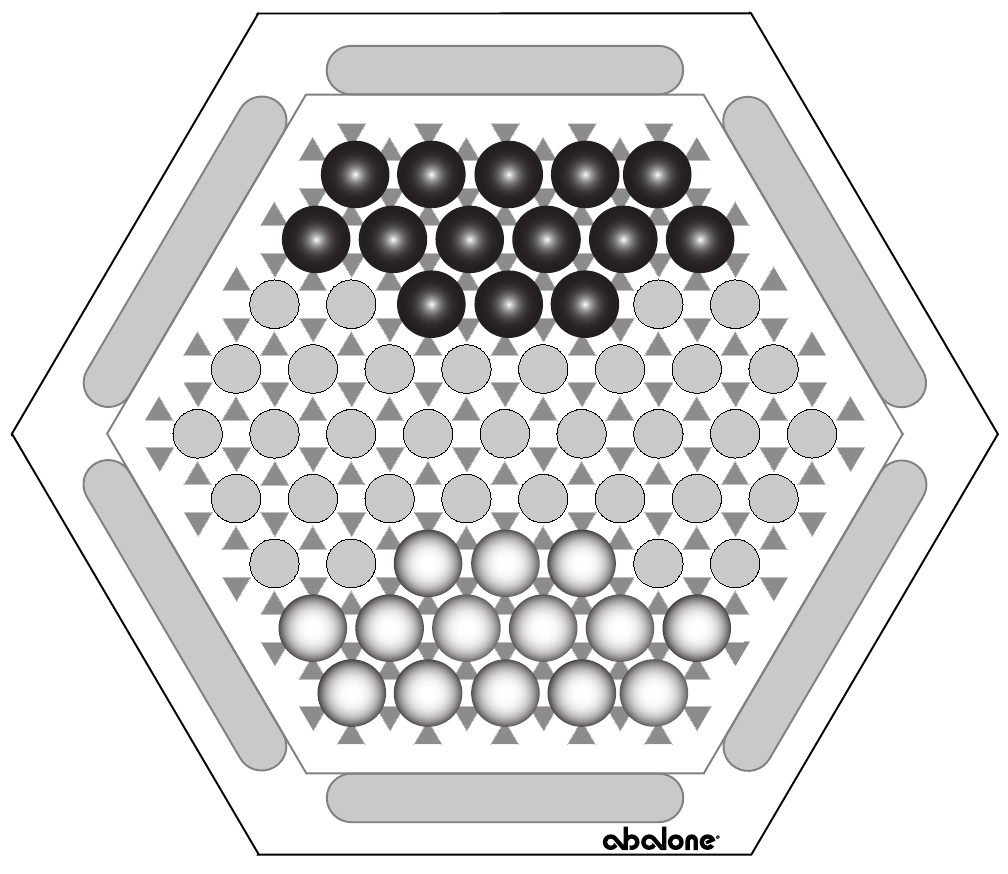
\includegraphics[width=3cm, keepaspectratio]{rules_starting_position.png}
    }
    \hfill
    \subfloat["In-line" moves]{
        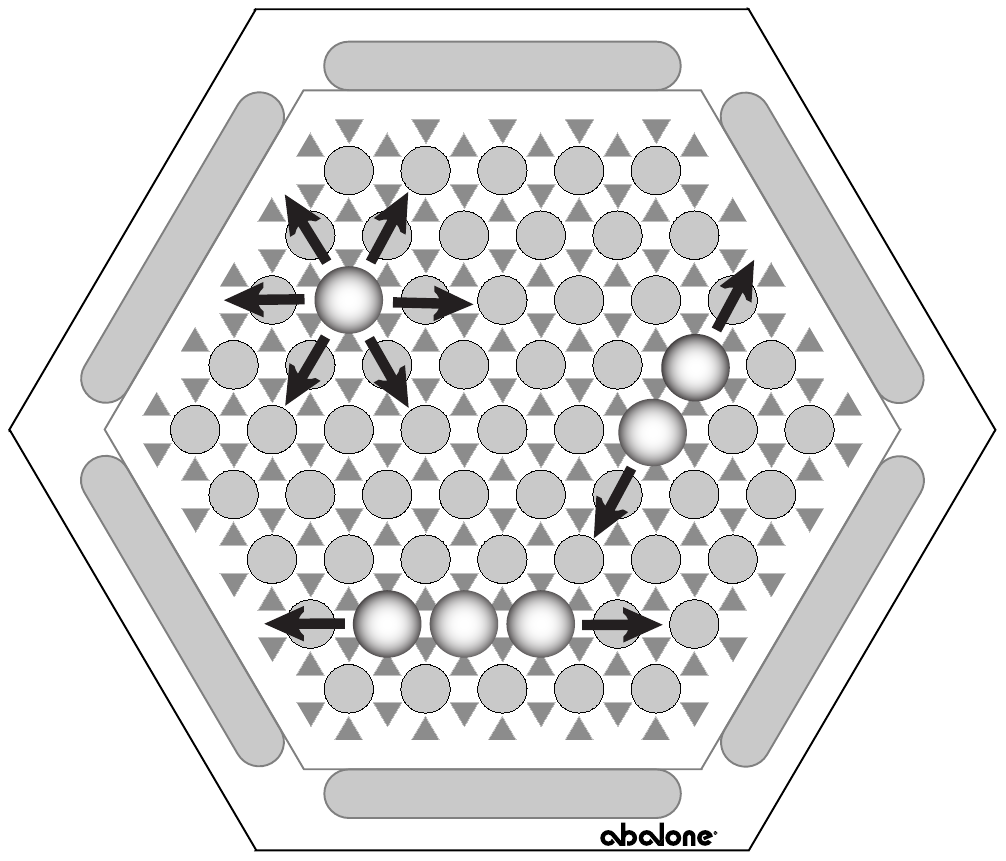
\includegraphics[width=3cm, keepaspectratio]{rules_inline_move.png}
    }
    \hfill
    \subfloat["Side-step" moves]{
        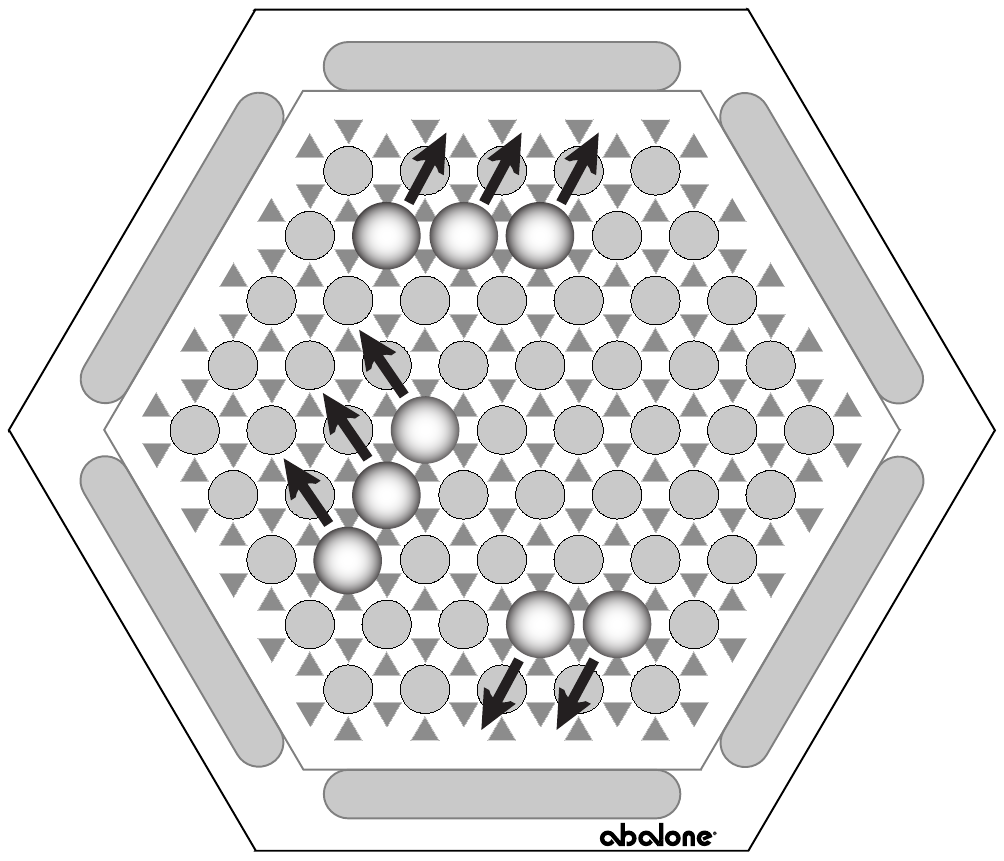
\includegraphics[width=3cm, keepaspectratio]{rules_side_step_move.png}
    }
    \caption{Basic moves \cite{abalone_sa_abalone_nodate}}
    \label{basics}
\end{figure}

A move pushing the opponent's marbles is called "sumito" and comes in three variations, as shown by figure \ref{sumito}. Essentially, the player has to push with superior numbers and the opponent's marbles can not be blocked. This is the game mechanic that allows for pushing the marbles out of the game and winning.

\begin{figure}[!h]
    \centering
    \subfloat["2-push-1" sumito]{
        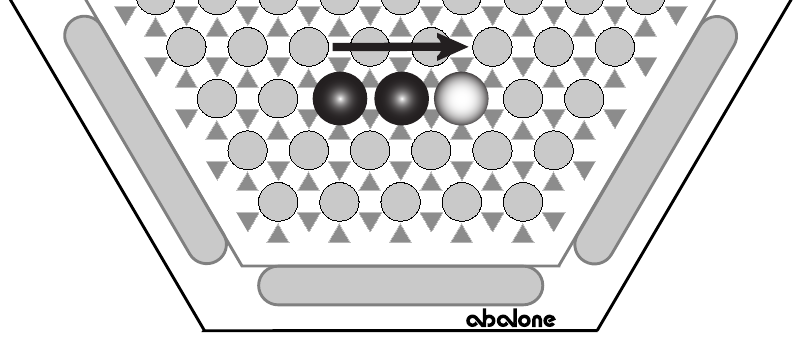
\includegraphics[width=3cm, keepaspectratio]{rules_2-push-1_sumito.png}
    }
    \hfill
    \subfloat["3-push-1" sumito]{
        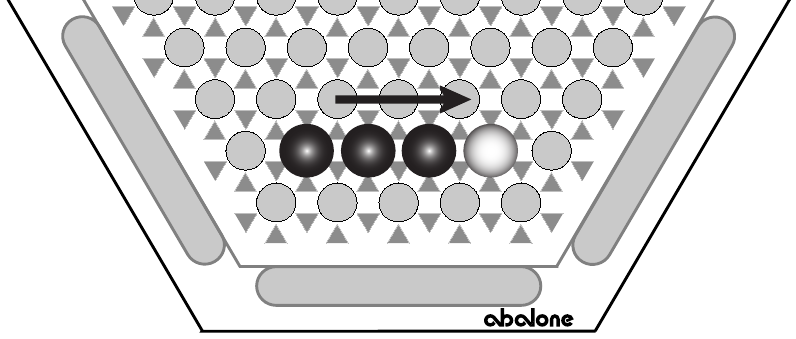
\includegraphics[width=3cm, keepaspectratio]{rules_3-push-1_sumito.png}
    }
    \hfill
    \subfloat["3-push-2" sumito]{
        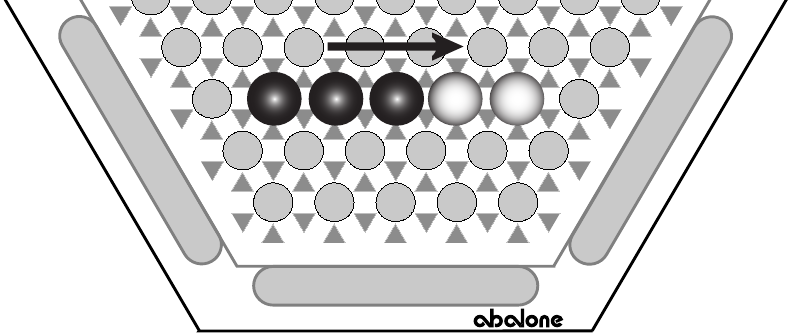
\includegraphics[width=3cm, keepaspectratio]{rules_3-push-2_sumito.png}
    }
    \caption{Sumito positions allow pushing the opponent's marbles \cite{abalone_sa_abalone_nodate}}
    \label{sumito}
\end{figure}

\subsection{Abalone complexity}

An important characteristic of a game environment is its complexity, which can be described in two relevant dimensions.

\paragraph{State space complexity}

The state space is the collection of all possible states the agent can be in.\cite[p. 150]{russell_artificial_2021} For Abalone this means we have to consider all possible board configurations with different numbers of marbles present. Additionally, we would have to correct duplicates that arise from the symmetries of the board. Ignoring this fact the following gives a good upper bound:

$$
    \sum_{k=8}^{14}\sum_{m=9}^{14}\frac{61!}{k!(61-k)!}\times\frac{(61-k)!}{m!((61-k)-m)!}
$$

\paragraph{Game tree complexity} The game tree defines the dependencies between board positions (nodes) and moves (edges). First we consider the branching factor (how many moves are possible in one position) of the game tree, which is on average 60. We combine that number with the height of the tree to get the total number of leaves. As the length of a game varies greatly, we use the average length of a game which is 87: $60^{87}$ \cite{lemmens_constructing_2005}

\begin{figure}
    \centering
    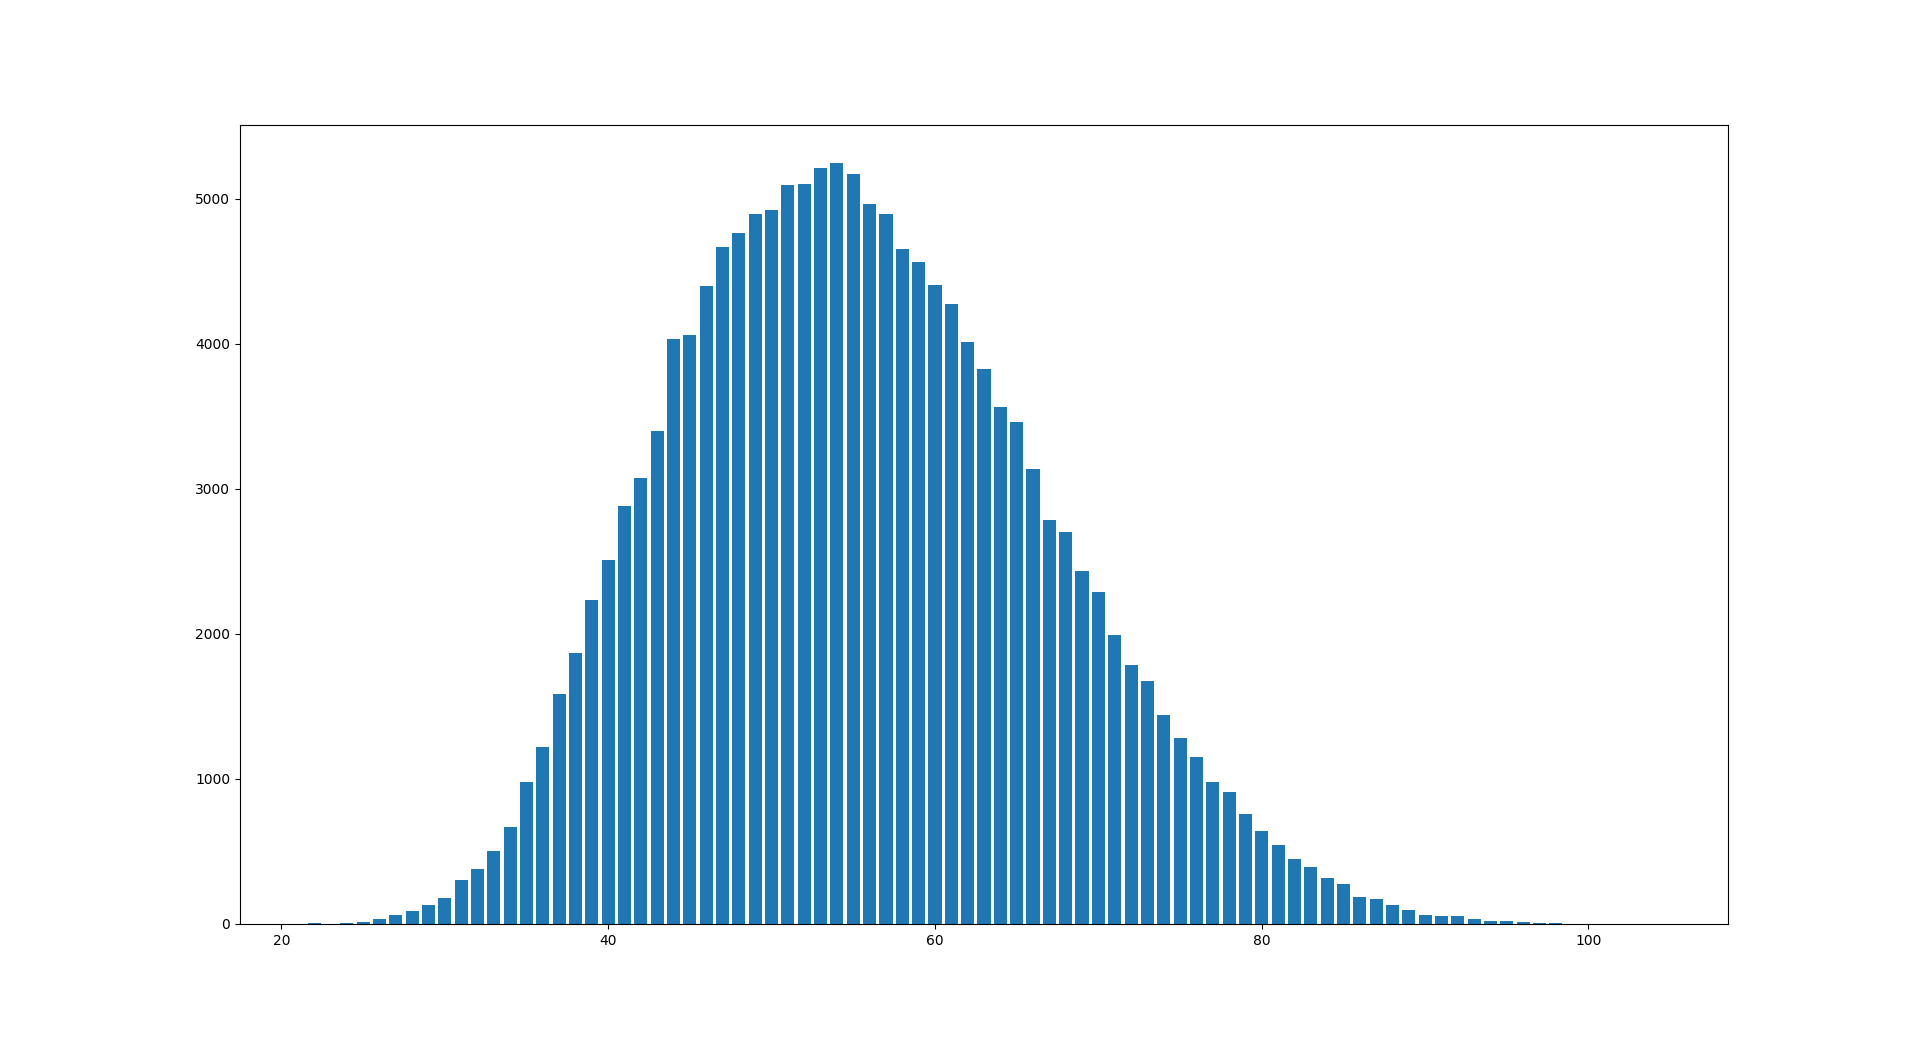
\includegraphics[width=7cm, keepaspectratio]{distribution_of_moves.png}
    \caption{Counts of moves available for random for random player in 5 games}
\end{figure}

Putting Abalone's complexity in relation with other popular games, its state space complexity is on the same level as Reversi, whilst its game tree surpasses chess in complexity (c.f. table \ref{complexity_table})

\begin{table}
    \begin{center}
        \begin{tabular}{ | c | c | c | }
            \hline
            Game        & state-space complexity (log) & game-tree complexity (log) \\
            \hline
            Tic-tac-toe & 3                            & 5                          \\
            \hline
            Reversi     & 28                           & 58                         \\
            \hline
            Chess       & 46                           & 123                        \\
            \hline
            Abalone     & 24                           & 154                        \\
            \hline
            Go          & 172                          & 360                        \\
            \hline
        \end{tabular}
    \end{center}
    \caption{Abalone in comparison with other games \cite{chorus_implementing_2009}}
    \label{complexity_table}
\end{table}